\section{Network}

For one neuron there is one output value so we can easily see that one is not enough to solve many problems. Combining neurons into networks and layers will make them more useful. But one single neuron is still able to solve some class of problems.

\begin{wrapfigure}{r}{0.3\textwidth}
    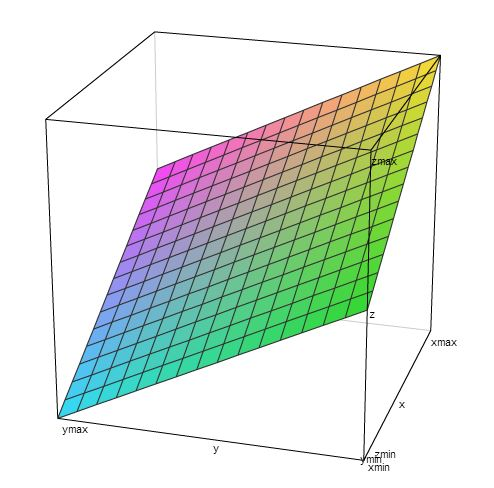
\includegraphics[width=0.32\textwidth]{Media/Plane.png}
    \caption{Single neuron plane}
    \label{fig:SingleNeuronPlane}
\end{wrapfigure}

Typically each neuron has one constant input value. Graphical interpretation of neuron can show why and also what class of problems can be solve with one neuron only.

Consider a neuron with three inputs $n = 3$ and with random weights $w_n$. So we have four axis, three for input data and one to show neuron output. Without one constant input graph of such neuron would be just a random set of points in 4D space.

But if we set one of the inputs constant then we will have only three axis, two for data and one for output value. Because of this one constant input instead of set of random points we will obtain 3D plane (\hyperref[fig:SingleNeuronPlane]{Figure \ref{fig:SingleNeuronPlane}}).

So our single neuron is able to model a $n$D planes. Such plane allows us to distinguish between three possibilities: data are greater then model, smaller or equal. It is enough to solve all linearly separable problems (e.g. logical AND, OR functions). But not all of the problems are linearly separable.


\subsection{Layers}

Before solving non linearly separable problems it have to be shown how more then one output can be obtain.

By putting same input values into multiple neurons with different set of weights $w_n$ a~more then one output can be obtain. Of course the single constant input still need to be provide for each of the neurons.

There are no differences between just using three separate neurons with different weights. So neurons in such configuration cannot solve problems beyond single neuron capabilities.

\begin{figure}[!h]
    \centering
    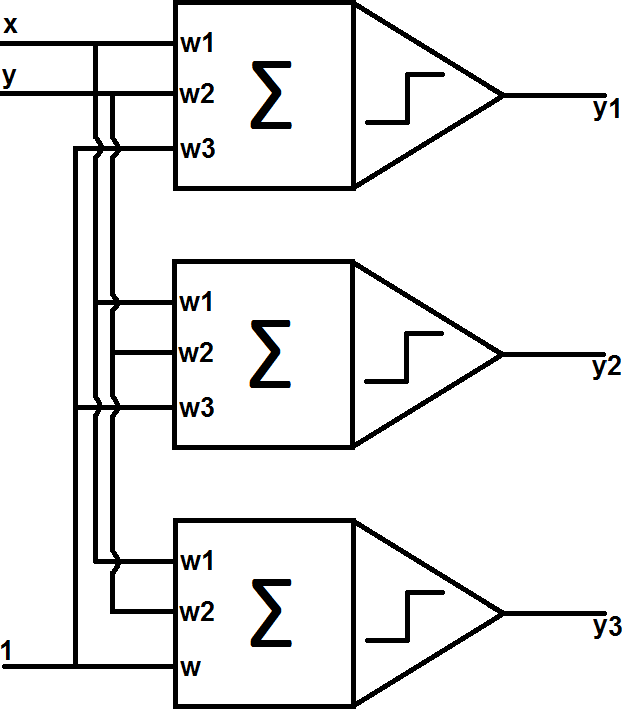
\includegraphics[scale=0.27]{Media/Layer.png}
    \caption[One layer of neurons]{One layer of neurons - two inputs with common constant one}
    \label{fig:OneNeuronsLayer}
\end{figure}

\newpage

\subsection{MLNN/PLP}

\begin{figure}[!h]
    \centering
    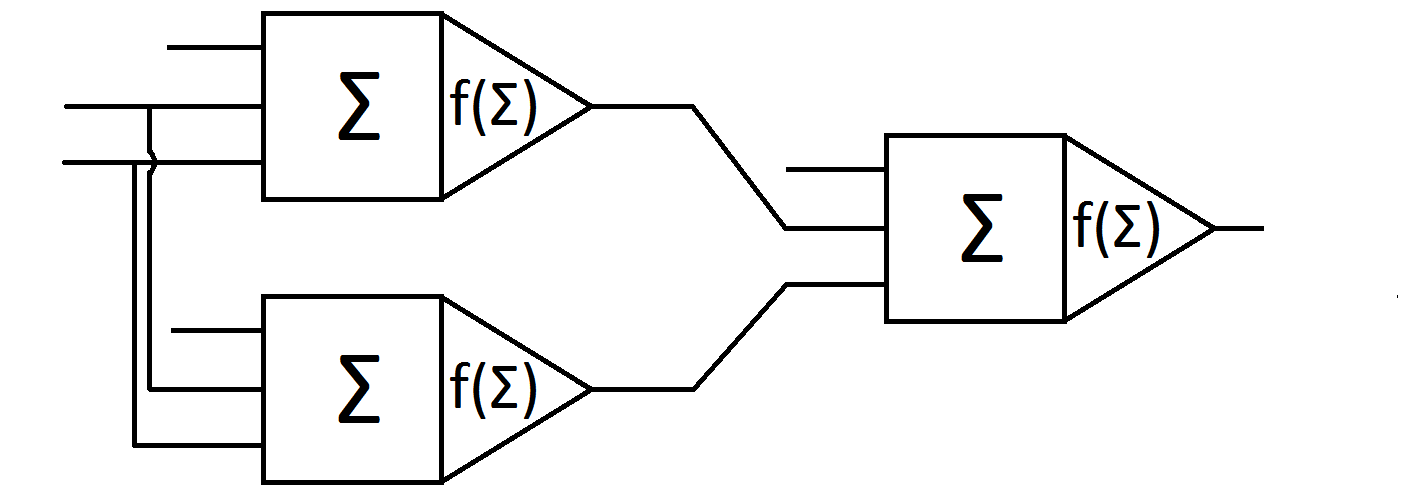
\includegraphics[scale=0.2]{Media/MLN.png}
    \caption[Multilayer network]{Very simple multilayer network}
    \label{fig:MLN}
\end{figure}

Non linearly separable problems can be solve by connecting multiple layers of neurons. \hyperref[fig:MLN]{Figure \ref{fig:MLN}} shows the simplest possible structure of \textit{Multilayer Perceptron}. Such structure is called \textit{Multilayer perceptron} or \textit{Feedforward neural network} or just \textit{Multilayer neural network}.

\textit{Feedforward neural network} is in our case the best naming convention because it tells exactly how each layer is connected. \textit{Feedforward} means that each output signal is connected only to next layer input. So no recursive connections, loops etc. Such network structure is most popular because we now how to train neurons in that structure. More about that in next \hyperref[sec:Training]{section}.

\begin{wrapfigure}[14]{r}{0.3\textwidth}
    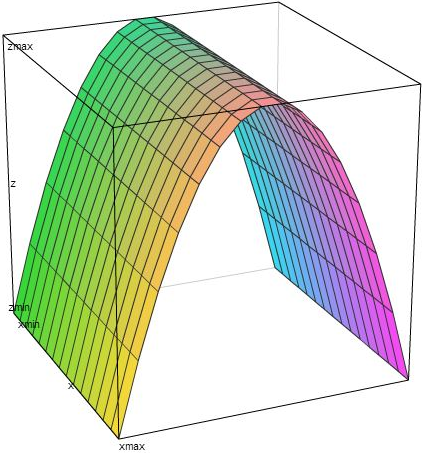
\includegraphics[width=0.32\textwidth]{Media/Bridge.png}
    \caption{Graph of three neurons combined in two layer structure}
    \label{fig:BridgeGraph}
\end{wrapfigure}

In general each multilayer network can be divided into three parts \cite{mlpPawelRosczak,mlpFSaC,fsmlpDwrSkrMk}:
\begin{itemize}
    \item \label{InputLayer} Input layer - used to prepare input data for network e.g. scaling or changing data distribution;
    \item \label{HiddenLayer} Hidden layers - actual \textit{feedforward network} with neurons; 
    \item \label{OutputLayer} Output layer - provides output data, can do some additional output preparation e.g. rescaling, swapping data;
\end{itemize}

\textit{Input layer} is in many cases omitted as well as \textit{output layer}.

The most important \textit{hidden layer} in \textit{feedforward network} has only one rule: \textit{connect output from $m$ layer to $m+1$ layer}. Not all of the output has to be connected to all neurons in next layer but this is usually the case. Still each of the neurons has to have its one constant input. Graph of such network (\hyperref[fig:BridgeGraph]{figure \ref{fig:BridgeGraph}}) will show why non linearly separable problems now can be model by such network.

\newpage
Now there is a question how many neurons and layers is needed. \\ There are two simple rules \cite{mlpPawelRosczak}:
\begin{enumerate}[topsep=8pt,itemsep=-1ex,partopsep=1ex,parsep=1ex]
    \item As small number of layers as possible
    \item As small number of neurons as possible
\end{enumerate}
And there are many approaches to solve this problem:
\begin{enumerate}[topsep=8pt,itemsep=-1ex,partopsep=1ex,parsep=1ex]
    \item Analytical calculations
    \item Building network from small number of neurons and measuring results
    \item Building network from large number of neurons and measuring results
    \item Generic algorithms
    \item Using theoretical knowledge about the problem
\end{enumerate}
None of this methods will be discussed here.

\begin{figure}[!h]
    \centering
    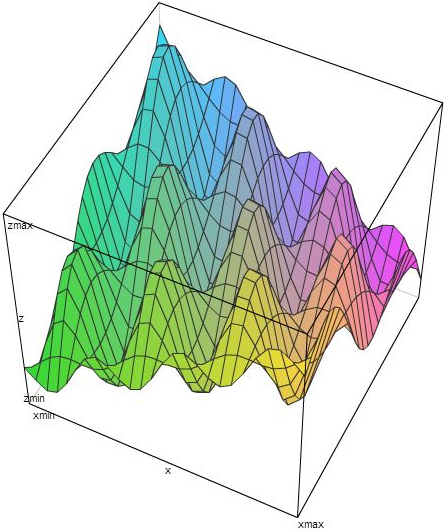
\includegraphics[scale=0.8]{Media/SolutionGraph.png}
    \caption{Complicated model modeled by MLP}
    \label{fig:SolutionGraph}
\end{figure}

\newpage
\subsection{Training}
\label{sec:Training}

Now the EBP\textit{(Error Back Propagation)} algorithm will be discussed \cite{mlpPawelRosczak,mlpFSaC,fsmlpDwrSkrMk,sRpNAI369}.
Training of multilayer network is numerical optimization of goal function $Q(k)$ where EBP algorithm in one of the gradient based methods.

\begin{mycapequ}[!ht]
    $$ {w_i}^{(n)}(k) = {w_i}^{(n)}(k-1)-\alpha\frac{\partial Q(k)}{{w_i}^{(n)}} $$
    \caption{Error Back Propagation \cite{mlpPawelRosczak}}
    \label{formula:EBP}
\end{mycapequ}

Using this formula we will for each iteration $k$ modify previous weight ${w_i}^{(n)}(k-1)$ of $i$ neuron in $n$ layer by negative gradient $\displaystyle{\alpha\frac{\partial Q(k)}{{w_i}^{(n)}}}$ where $\alpha$ is \textit{learn factor} (determine \textit{speed} of learning).
Goal function $Q(k)$ is usually square of the network result error.

\ 


To know network error the sample set with both inputs and results is needed. Such form of network training is called supervised. Creating good sample set is a~very large topic and wont be discussed here.
